\documentclass[12pt]{article}

\usepackage{sbc-template}
\usepackage{graphicx,url}
\usepackage{xcolor}
\usepackage{placeins}
\usepackage{subcaption}
\usepackage[utf8]{inputenc}
\usepackage[english]{babel}


\sloppy

\title{Developing and Evaluating Predictive Models for Chronic Kidney Disease Detection}

\author{Ariel M. Fagundes\inst{1}, Rodrigo Mancuso\inst{1}, Anderson Gonçalves\inst{1} }

\address{Instituto de Informática -- Universidade Federal do Rio Grande do Sul
  (UFRGS)\\
  Caixa Postal 15.064 -- 91.501-970 -- Porto Alegre -- RS -- Brazil
  \email{\{ariel,rodrigo,anderson\}@inf.ufrgs.br}
}

\begin{document}

\maketitle

\begin{abstract}

Chronic Kidney Disease (CKD) is a relevant public health problem in which early diagnosis may
improve patient outcomes. This work evaluates machine learning models for CKD prediction using the
UCI CKD dataset \cite{risk_factor_prediction_of_chronic_kidney_disease_857}. Random Forest, SVM,
KNN, Naive Bayes, and Decision Tree were evaluated with balancing and dimensionality reduction
techniques, including SMOTE, Random Under Sampling, SMOTE + Tomek Links, PCA, SelectKBest,
SelectFromModel, and RFECV. Models were assessed using accuracy, precision, recall, and F1-score.
The best-performing model was further analyzed using explainability and interpretability techniques
to provide insights into the decision-making process and feature importance for CKD prediction.

\end{abstract}

% ===== Sections =====

\section{Introduction}

\todo{
\begin{itemize}
    \item Present the context of the problem and explain its practical relevance.
    \item Provide background information necessary to understand the problem domain.
    \item Briefly review related work or existing approaches to similar problems.
    \item Clearly define the problem being addressed.
    \item State the main objectives of the study.
    \item Highlight the expected contributions of the work.
\end{itemize}
}

Chronic Kidney Disease (CKD) represents a significant public health challenge
characterized by the progressive loss of renal function. Early identification of
individuals at risk is essential for timely intervention and improved clinical
outcomes. In recent years, machine learning approaches have emerged as promising
tools for supporting disease prediction tasks through the analysis of structured
clinical and laboratory data. Supervised classification methods, in particular,
have demonstrated strong potential for identifying patterns associated with
chronic diseases and supporting data-driven healthcare analysis
\cite{obermeyer2016,deo2015}.

The development of reliable predictive models for CKD involves multiple stages
of the machine learning workflow, including exploratory data analysis,
preprocessing, model selection, hyperparameter optimization, and model
interpretation. In clinical datasets, preprocessing techniques such as class
balancing and dimensionality reduction are frequently employed to address issues
including class imbalance, noisy attributes, and feature redundancy
\cite{he2009imbalanced,chawla2002smote}.
Additionally, robust evaluation strategies are necessary to ensure fair model
comparison and reproducibility of experimental results.

Prior work has demonstrated the applicability of machine learning to CKD
prediction using the same dataset adopted in this study. Islam et al.
\cite{inproceedings} evaluated Naive Bayes, Random Forest, Logistic Regression,
Decision Stump, and Linear Regression models for CKD risk factor prediction,
establishing a baseline for algorithm comparison on this data. Building on this
prior work, the present study extends the evaluation to a broader set of
algorithms, including Support Vector Machines (SVM) and K-Nearest Neighbors
(KNN), and incorporates class balancing and dimensionality reduction strategies
not explored in that work. Furthermore, explainability methods such as SHAP and
LIME have gained importance in healthcare-related applications by improving
transparency and supporting interpretation of model behavior.

In this context, this work investigates the impact of different preprocessing
and model optimization strategies on CKD prediction using the UCI Chronic Kidney
Disease dataset \cite{risk_factor_prediction_of_chronic_kidney_disease_857}. The
proposed workflow includes exploratory data analysis, evaluation of multiple
classification algorithms, application of balancing and dimensionality reduction
techniques, hyperparameter optimization using nested cross-validation, and
interpretability analysis of the final model. Experiments were conducted using
Stratified 5-Fold Cross-Validation to ensure consistent evaluation conditions.

The main objectives of this study are: (i) to compare the predictive performance
of different supervised learning algorithms for CKD prediction; (ii) to evaluate
the impact of class balancing and dimensionality reduction techniques on model
performance; (iii) to investigate hyperparameter optimization strategies for the
best-performing model; and (iv) to analyze model interpretability using feature
importance, permutation importance, SHAP, and LIME. Together, these objectives
aim to contribute a reproducible experimental framework for CKD classification
that pairs rigorous comparative evaluation of diverse supervised learning
algorithms with transparent post-hoc model interpretation.


\section{Methodology}

This study follows a machine learning pipeline composed of exploratory data analysis,
preprocessing, model training and validation, and interpretation of results.
Each step is described in detail below.

\subsection{Exploratory Data Analysis (EDA)}

\todo{
\begin{itemize}
    \item Describe the main characteristics of the dataset, including the number of instances, number
        and types of attributes, and the definition of the target variable.
    \item Present the distribution of the target attribute and discuss possible class imbalance issues.
    \item Report the presence of patterns, anomalies, or inconsistencies observed in the dataset, such
        as outliers, missing values, duplicated records, or irregular values.
    \item Present visualizations and statistical summaries used to support the exploratory analysis
        (e.g., histograms, boxplots, correlation matrices, descriptive statistics).
    \item Discuss relationships between attributes and identify possible redundant or highly correlated features.
    \item Highlight attributes or instances that were identified as potentially irrelevant, redundant, or problematic.
    \item Summarize the main findings obtained from the exploratory analysis.
    \item Based on these findings, describe the data quality issues identified and motivate the preprocessing steps
        required for data preparation.
\end{itemize}
}

\subsection{Data Preprocessing}

\todo{
\begin{itemize}
    \item Describe the preprocessing steps applied to the dataset based on the issues identified during the
        exploratory data analysis.
    \item Explain the criteria used to remove or modify attributes or instances considered
        irrelevant, redundant, or inconsistent.
    \item Describe how missing values were handled and justify the chosen strategy.
    \item Report how outliers were treated and explain the reasoning behind the adopted approach.
    \item Describe any normalization or standardization procedures applied to numerical attributes.
    \item Explain how categorical variables were encoded and justify the selected encoding method.
    \item Describe any techniques used to address class imbalance, when applicable.
    \item Report the use of dimensionality reduction or feature selection methods, if applied,
        including the criteria used.
    \item Explain how preprocessing steps were incorporated into the modeling workflow.
    \item If no preprocessing was required, explicitly state this and justify the decision based on the data analysis.
\end{itemize}
}

\subsection{Definition of the Approach, Algorithms, and Evaluation Strategy}

\todo{
\begin{itemize}
    \item Describe the overall machine learning approach adopted to address the problem, including
        the type of learning task (e.g., classification or regression).
    \item Present the set of supervised learning algorithms selected for the study and justify their
        inclusion based on their characteristics and suitability for the problem.
    \item Highlight the diversity of the selected algorithms in terms of modeling strategies or inductive biases.
    \item Describe the performance evaluation metrics used to assess model performance, explaining
        their relevance to the problem context.
    \item Indicate the primary metric used as the main criterion for model selection and optimization,
        and justify this choice.
    \item Describe the strategy used to divide the dataset into training, validation, and testing subsets.
    \item Explain the evaluation methodology adopted (e.g., holdout validation or cross-validation),
        including how it contributes to reliable model assessment.
    \item Justify the methodological choices made in this stage based on best practices or characteristics
        of the dataset and problem.
\end{itemize}
}

\subsection{Model Training, Hyperparameter Tuning, and Validation}

\todo{
\begin{itemize}
    \item Describe how the selected models were trained according to the previously defined experimental setup.
    \item Report whether an initial comparison of algorithms (e.g., spot-checking) was performed and describe its
        purpose in guiding the selection of promising models.
    \item Describe the hyperparameter tuning procedures applied to the selected models, including the search strategies used.
    \item Explain how data separation was maintained throughout the training and validation process to avoid data leakage.
    \item Describe how consistency across experiments was ensured, including the use of identical data partitions when
        comparing different algorithms.
    \item Report the use of repeated experiments or multiple runs, when applicable, to improve the reliability of
        the obtained results.
    \item Describe the steps taken to ensure reproducibility of the experiments, such as the use of fixed random seeds.
    \item Summarize how model performance was recorded and organized for subsequent analysis.
\end{itemize}
}

\subsection{Model Interpretation and Analysis}

After model selection, post-hoc explainability methods were applied to the
selected CKD classifier. This interpretation stage was not used to train or
select the model; instead, it was used to analyze the behavior of the selected
model after the predictive modeling workflow had been completed. The
explainability analysis combined model-specific feature importance, permutation
feature importance, SHAP-based summaries, SHAP waterfall plots, and LIME local
explanations \cite{fisher2019modelreliance,lundberg2017shap,ribeiro2016lime}.
Because the selected classifier was a Random Forest model
\cite{breiman2001randomforests}, native feature importance was also reported as
a model-specific global explanation.

Global explanations were used to identify features most associated with the
model predictions across the test set, while local explanations were used to
inspect representative individual predictions. SHAP values were interpreted
with respect to the configured explained class, \texttt{ckd}; positive SHAP
values indicate increased support for that class, whereas negative SHAP values
indicate reduced support for that class. These explanations were treated as
model-dependent interpretability evidence and not as causal clinical
conclusions \cite{molnar2022interpretable,doshivelez2017interpretable}.


\section{Results}

\subsection{Model Comparison}

The initial model comparison evaluated KNN, Decision Tree, Random Forest, SVM,
and Naive Bayes using stratified 5-fold cross-validation. The same
preprocessing workflow was applied inside each fold to reduce the risk of data
leakage. At this stage, no dimensionality-reduction or balancing strategy was
applied, establishing a baseline for the subsequent preprocessing experiments.

Random Forest obtained the best overall performance among the evaluated
classifiers, with overall accuracy of 0.9950 and macro-F1 of 0.9945. Because
the encoded labels map \texttt{ckd} to 0 and \texttt{notckd} to 1, the
class-wise metrics were reported explicitly instead of relying only on the
default positive class used by scikit-learn. For CKD, Random Forest obtained
precision of 0.9922, recall of 1.0000, and F1-score of 0.9961; for NOTCKD, it
obtained precision of 1.0000, recall of 0.9861, and F1-score of 0.9930.

SVM and Naive Bayes also performed well, but Random Forest achieved the
strongest overall metric profile. These results address the first objective of
the study by showing that Random Forest was the best-performing classifier
among the evaluated supervised learning models. For this reason, it was used as
the reference model in the balancing, dimensionality-reduction, optimization,
and interpretability stages. Table~\ref{tab:model_comparison} summarizes the
main metrics, while Figure~\ref{fig:model_comparison_results} presents the
F1-score distribution and ROC curves.

\begin{table}[!htbp]
\centering
\caption{Initial classifier comparison using no dimensionality reduction and no balancing.}
\label{tab:model_comparison}
\begin{tabular}{lcccc}
\hline
Model & Accuracy & Macro-F1 & CKD F1 & NOTCKD F1 \\
\hline
Random Forest & 0.9950 & 0.9945 & 0.9961 & 0.9930 \\
SVM & 0.9749 & 0.9732 & 0.9799 & 0.9664 \\
Decision Tree & 0.9598 & 0.9567 & 0.9683 & 0.9452 \\
Naive Bayes & 0.9548 & 0.9522 & 0.9633 & 0.9412 \\
KNN & 0.9447 & 0.9419 & 0.9547 & 0.9290 \\
\hline
\end{tabular}
\end{table}

\begin{figure}[!htbp]
\centering
\begin{subfigure}{0.48\linewidth}
\centering
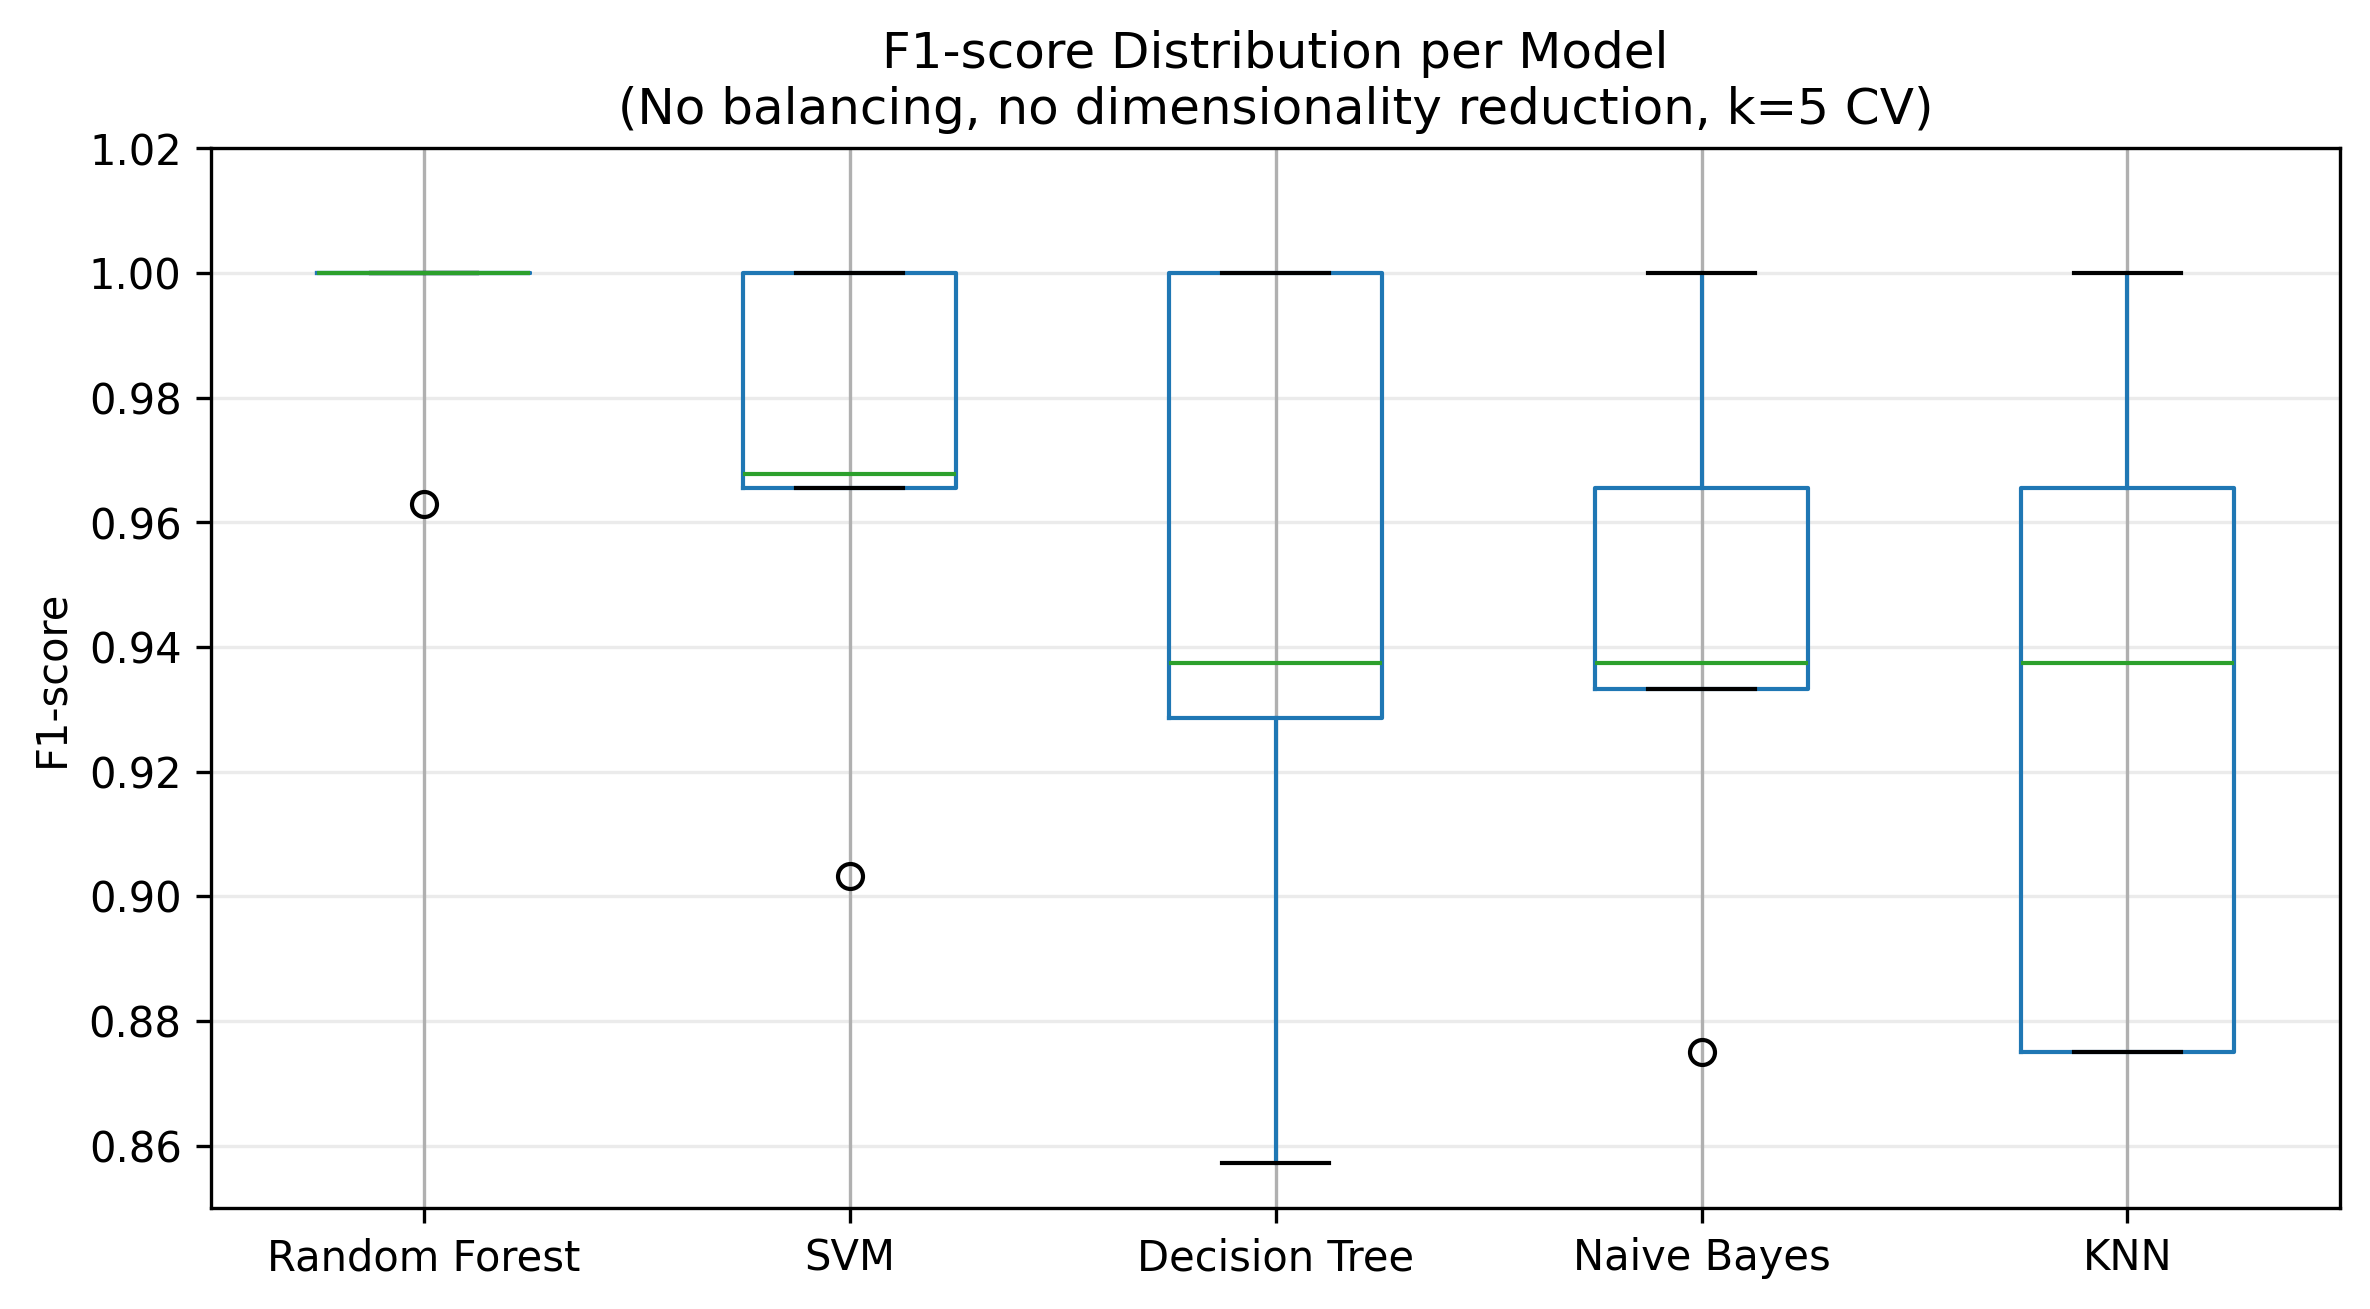
\includegraphics[width=\linewidth]{figures/model_comparison_no_dr_boxplot.png}
\caption{F1-score distribution.}
\end{subfigure}
\hfill
\begin{subfigure}{0.48\linewidth}
\centering
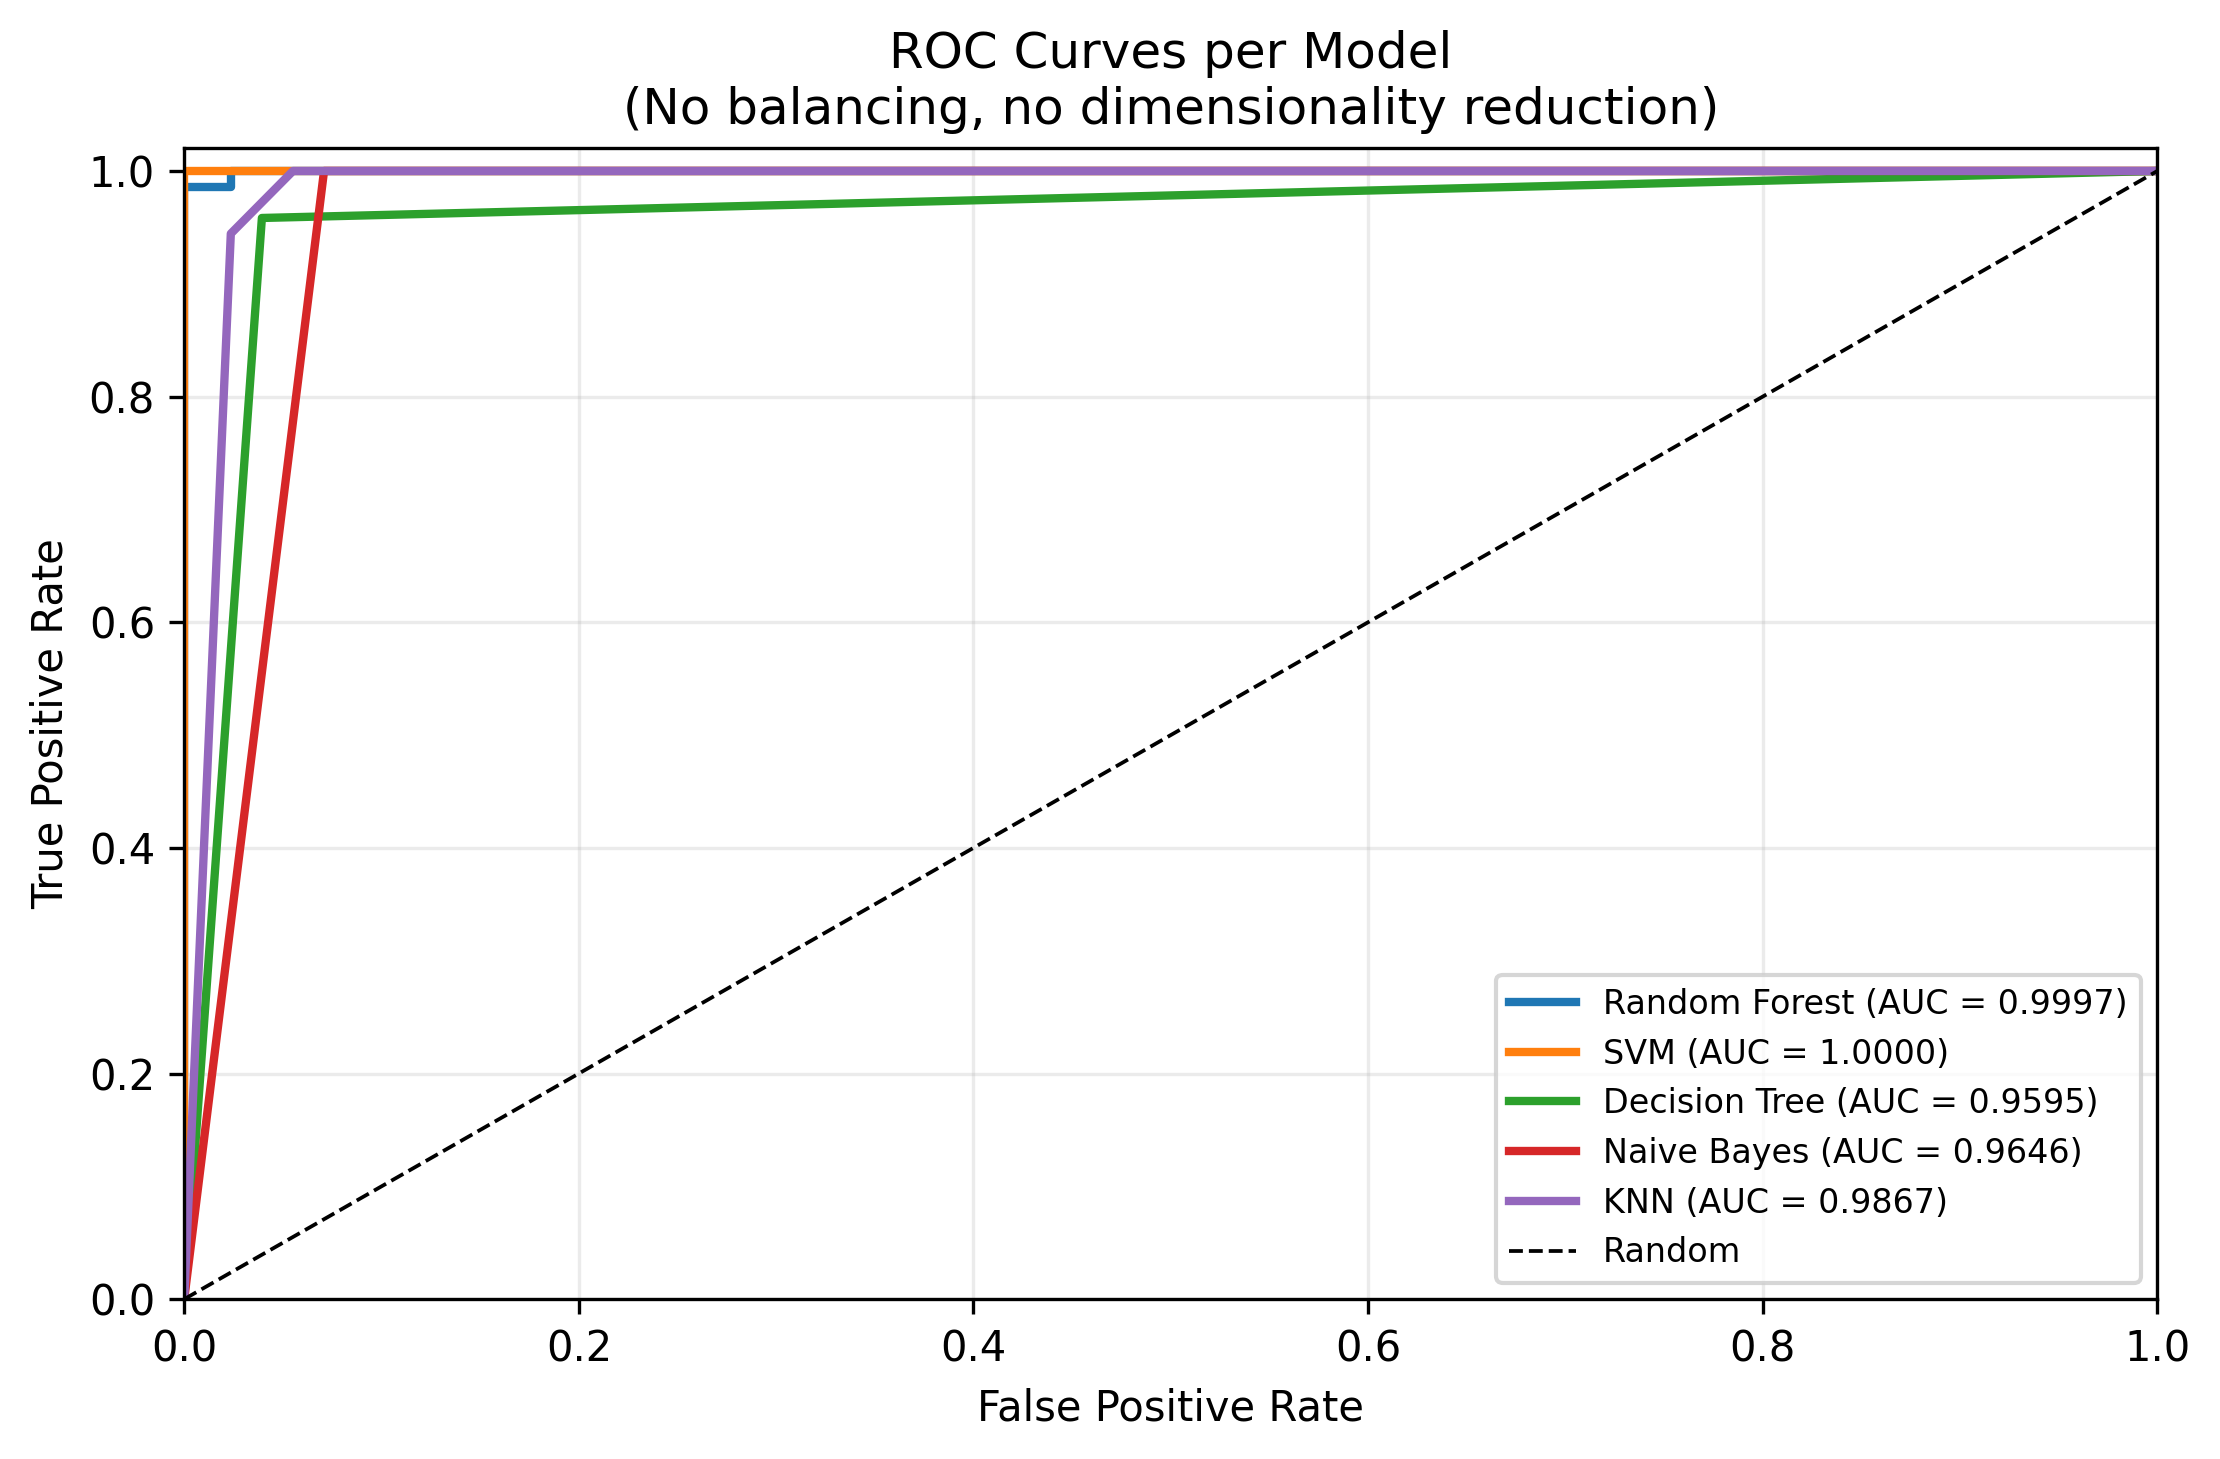
\includegraphics[width=\linewidth]{figures/model_comparison_no_dr_roc_curve.png}
\caption{ROC curves.}
\end{subfigure}
\caption{Initial model-comparison results.}
\label{fig:model_comparison_results}
\end{figure}

\FloatBarrier

\subsection{Balancing and Dimensionality Reduction}

The balancing experiments compared the original class distribution against
SMOTE, Random Under Sampling, and SMOTE combined with Tomek Links. Because the
dataset has only moderate imbalance, the balancing techniques did not improve
the average performance across models. The best average F1-score was obtained
without balancing, with F1-score of 0.9555 across the evaluated algorithms.
For Random Forest specifically, the F1-score remained 0.9926 for no balancing,
SMOTE, and SMOTE with Tomek Links, while Random Under Sampling reduced the
F1-score to 0.9867. Therefore, the final workflow did not include a balancing
step.

\begin{table}[!htbp]
\centering
\caption{Average results by balancing strategy across evaluated models.}
\label{tab:balancing_results}
\begin{tabular}{lcccc}
\hline
Strategy & Accuracy & Precision & Recall & F1-score \\
\hline
No balancing & 0.9658 & 0.9281 & 0.9886 & 0.9555 \\
SMOTE + Tomek Links & 0.9628 & 0.9219 & 0.9886 & 0.9518 \\
SMOTE & 0.9618 & 0.9193 & 0.9886 & 0.9506 \\
Random Under Sampling & 0.9537 & 0.9014 & 0.9914 & 0.9416 \\
\hline
\end{tabular}
\end{table}

Dimensionality-reduction experiments showed that PCA produced the strongest
average performance across the evaluated models. PCA retaining 90\% of the
variance achieved the best average F1-score across classifiers.

For Random Forest, PCA retaining 95\% of the variance produced the highest mean
F1-score. However, the difference from the no-dimensionality-reduction baseline
was only 0.0009. Since this gain was very small and
PCA reduces the direct traceability between model explanations and the original
clinical variables, the final workflow kept the no-PCA configuration.

\begin{table}[!htbp]
\centering
\caption{Random Forest results by dimensionality-reduction strategy.}
\label{tab:rf_dimensionality_reduction}
\begin{tabular}{lcccc}
\hline
Strategy & Accuracy & Precision & Recall & F1-score \\
\hline
PCA 95\% & 0.9950 & 0.9875 & 1.0000 & 0.9935 \\
No dimensionality reduction & 0.9949 & 1.0000 & 0.9857 & 0.9926 \\
PCA 90\% & 0.9900 & 0.9742 & 1.0000 & 0.9867 \\
Filter (mutual information) & 0.9899 & 0.9867 & 0.9857 & 0.9857 \\
Embedded Random Forest & 0.9899 & 0.9867 & 0.9857 & 0.9857 \\
Filter (ANOVA F-test) & 0.9847 & 0.9867 & 0.9714 & 0.9777 \\
Embedded LinearSVC & 0.9797 & 0.9857 & 0.9571 & 0.9703 \\
\hline
\end{tabular}
\end{table}

\begin{table}[!htbp]
\centering
\caption{Average ranking of dimensionality-reduction strategies across evaluated models.}
\label{tab:dr_average_ranking}
\begin{tabular}{lcccc}
\hline
Strategy & Accuracy & Precision & Recall & F1-score \\
\hline
PCA 90\% & 0.9759 & 0.9475 & 0.9914 & 0.9679 \\
PCA 95\% & 0.9749 & 0.9459 & 0.9914 & 0.9669 \\
Embedded Random Forest & 0.9719 & 0.9425 & 0.9886 & 0.9632 \\
Filter (mutual information) & 0.9718 & 0.9398 & 0.9886 & 0.9625 \\
Filter (ANOVA F-test) & 0.9708 & 0.9404 & 0.9857 & 0.9610 \\
No dimensionality reduction & 0.9658 & 0.9281 & 0.9886 & 0.9555 \\
Embedded LinearSVC & 0.9598 & 0.9217 & 0.9802 & 0.9475 \\
\hline
\end{tabular}
\end{table}

\FloatBarrier

\subsection{Hyperparameter Tuning and Final Model}

The Random Forest classifier was further evaluated using default parameters,
GridSearchCV, and RandomizedSearchCV under two preprocessing settings: no
dimensionality reduction and PCA retaining 95\% of the variance. The default
Random Forest configuration refers to the default parameters of the
scikit-learn version used in the experiments.

The tuning results showed that hyperparameter search did not provide a
meaningful gain over the default Random Forest configuration. With PCA 95\%,
GridSearchCV and the baseline configuration reached the same mean F1-score of
0.9935. Without PCA, the baseline, GridSearchCV, and the fine RandomizedSearchCV
configuration also reached the same mean F1-score of 0.9926.

Because the performance difference between the best PCA-based configuration and
the no-PCA Random Forest was only 0.0009 in mean F1-score, the final selected
model was the default Random Forest without balancing and without PCA. This
choice preserves near-identical predictive performance while avoiding the
additional pipeline complexity of PCA and hyperparameter search. It also keeps
the model easier to interpret using the original clinical attributes. The
hyperparameter-tuning ranking is summarized in
Table~\ref{tab:rf_hyperparameter_ranking}, and the supporting plots are shown
in Figure~\ref{fig:rf_hyperparameter_results}.

\begin{table}[!htbp]
\centering
\caption{Random Forest hyperparameter-tuning ranking.}
\label{tab:rf_hyperparameter_ranking}
\resizebox{\linewidth}{!}{%
\begin{tabular}{llcccc}
\hline
Preprocessing & Configuration & Accuracy & Precision & Recall & F1-score \\
\hline
PCA 95\% & GridSearchCV & 0.9950 & 0.9875 & 1.0000 & 0.9935 \\
PCA 95\% & Baseline & 0.9950 & 0.9875 & 1.0000 & 0.9935 \\
No DR & Baseline & 0.9949 & 1.0000 & 0.9857 & 0.9926 \\
No DR & GridSearchCV & 0.9949 & 1.0000 & 0.9857 & 0.9926 \\
No DR & RandomizedSearchCV fine & 0.9949 & 1.0000 & 0.9857 & 0.9926 \\
PCA 95\% & RandomizedSearchCV broad & 0.9900 & 0.9742 & 1.0000 & 0.9867 \\
PCA 95\% & RandomizedSearchCV fine & 0.9900 & 0.9742 & 1.0000 & 0.9867 \\
No DR & RandomizedSearchCV broad & 0.9899 & 0.9875 & 0.9857 & 0.9861 \\
\hline
\end{tabular}
}
\end{table}

\begin{figure}[!htbp]
\centering
\begin{subfigure}{0.48\linewidth}
\centering
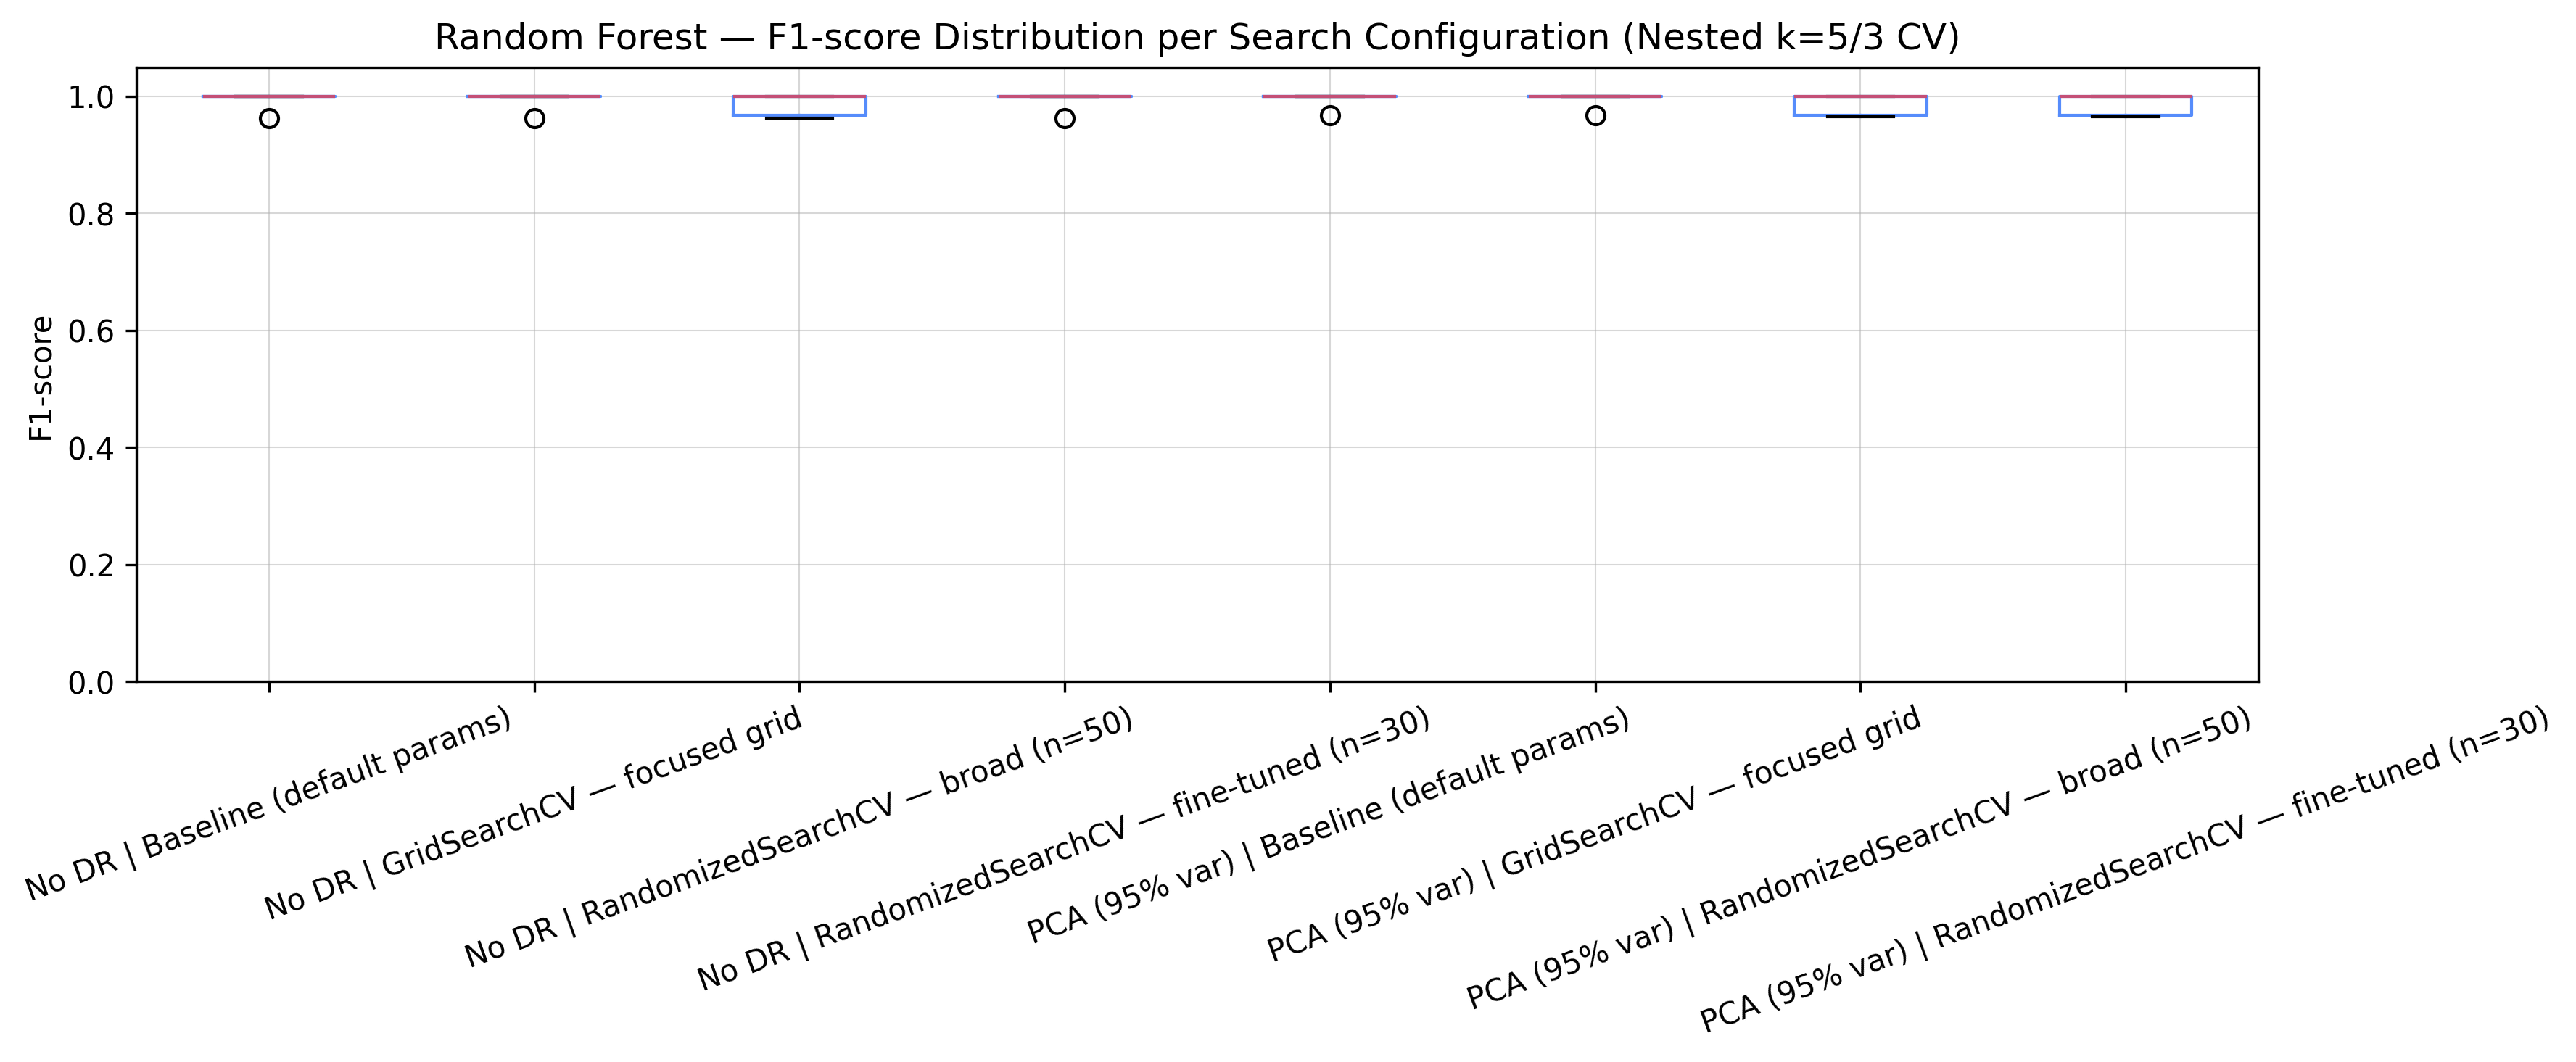
\includegraphics[width=\linewidth]{figures/optimize_rf_hyperparameters_boxplot.png}
\caption{F1-score distribution.}
\end{subfigure}
\hfill
\begin{subfigure}{0.48\linewidth}
\centering
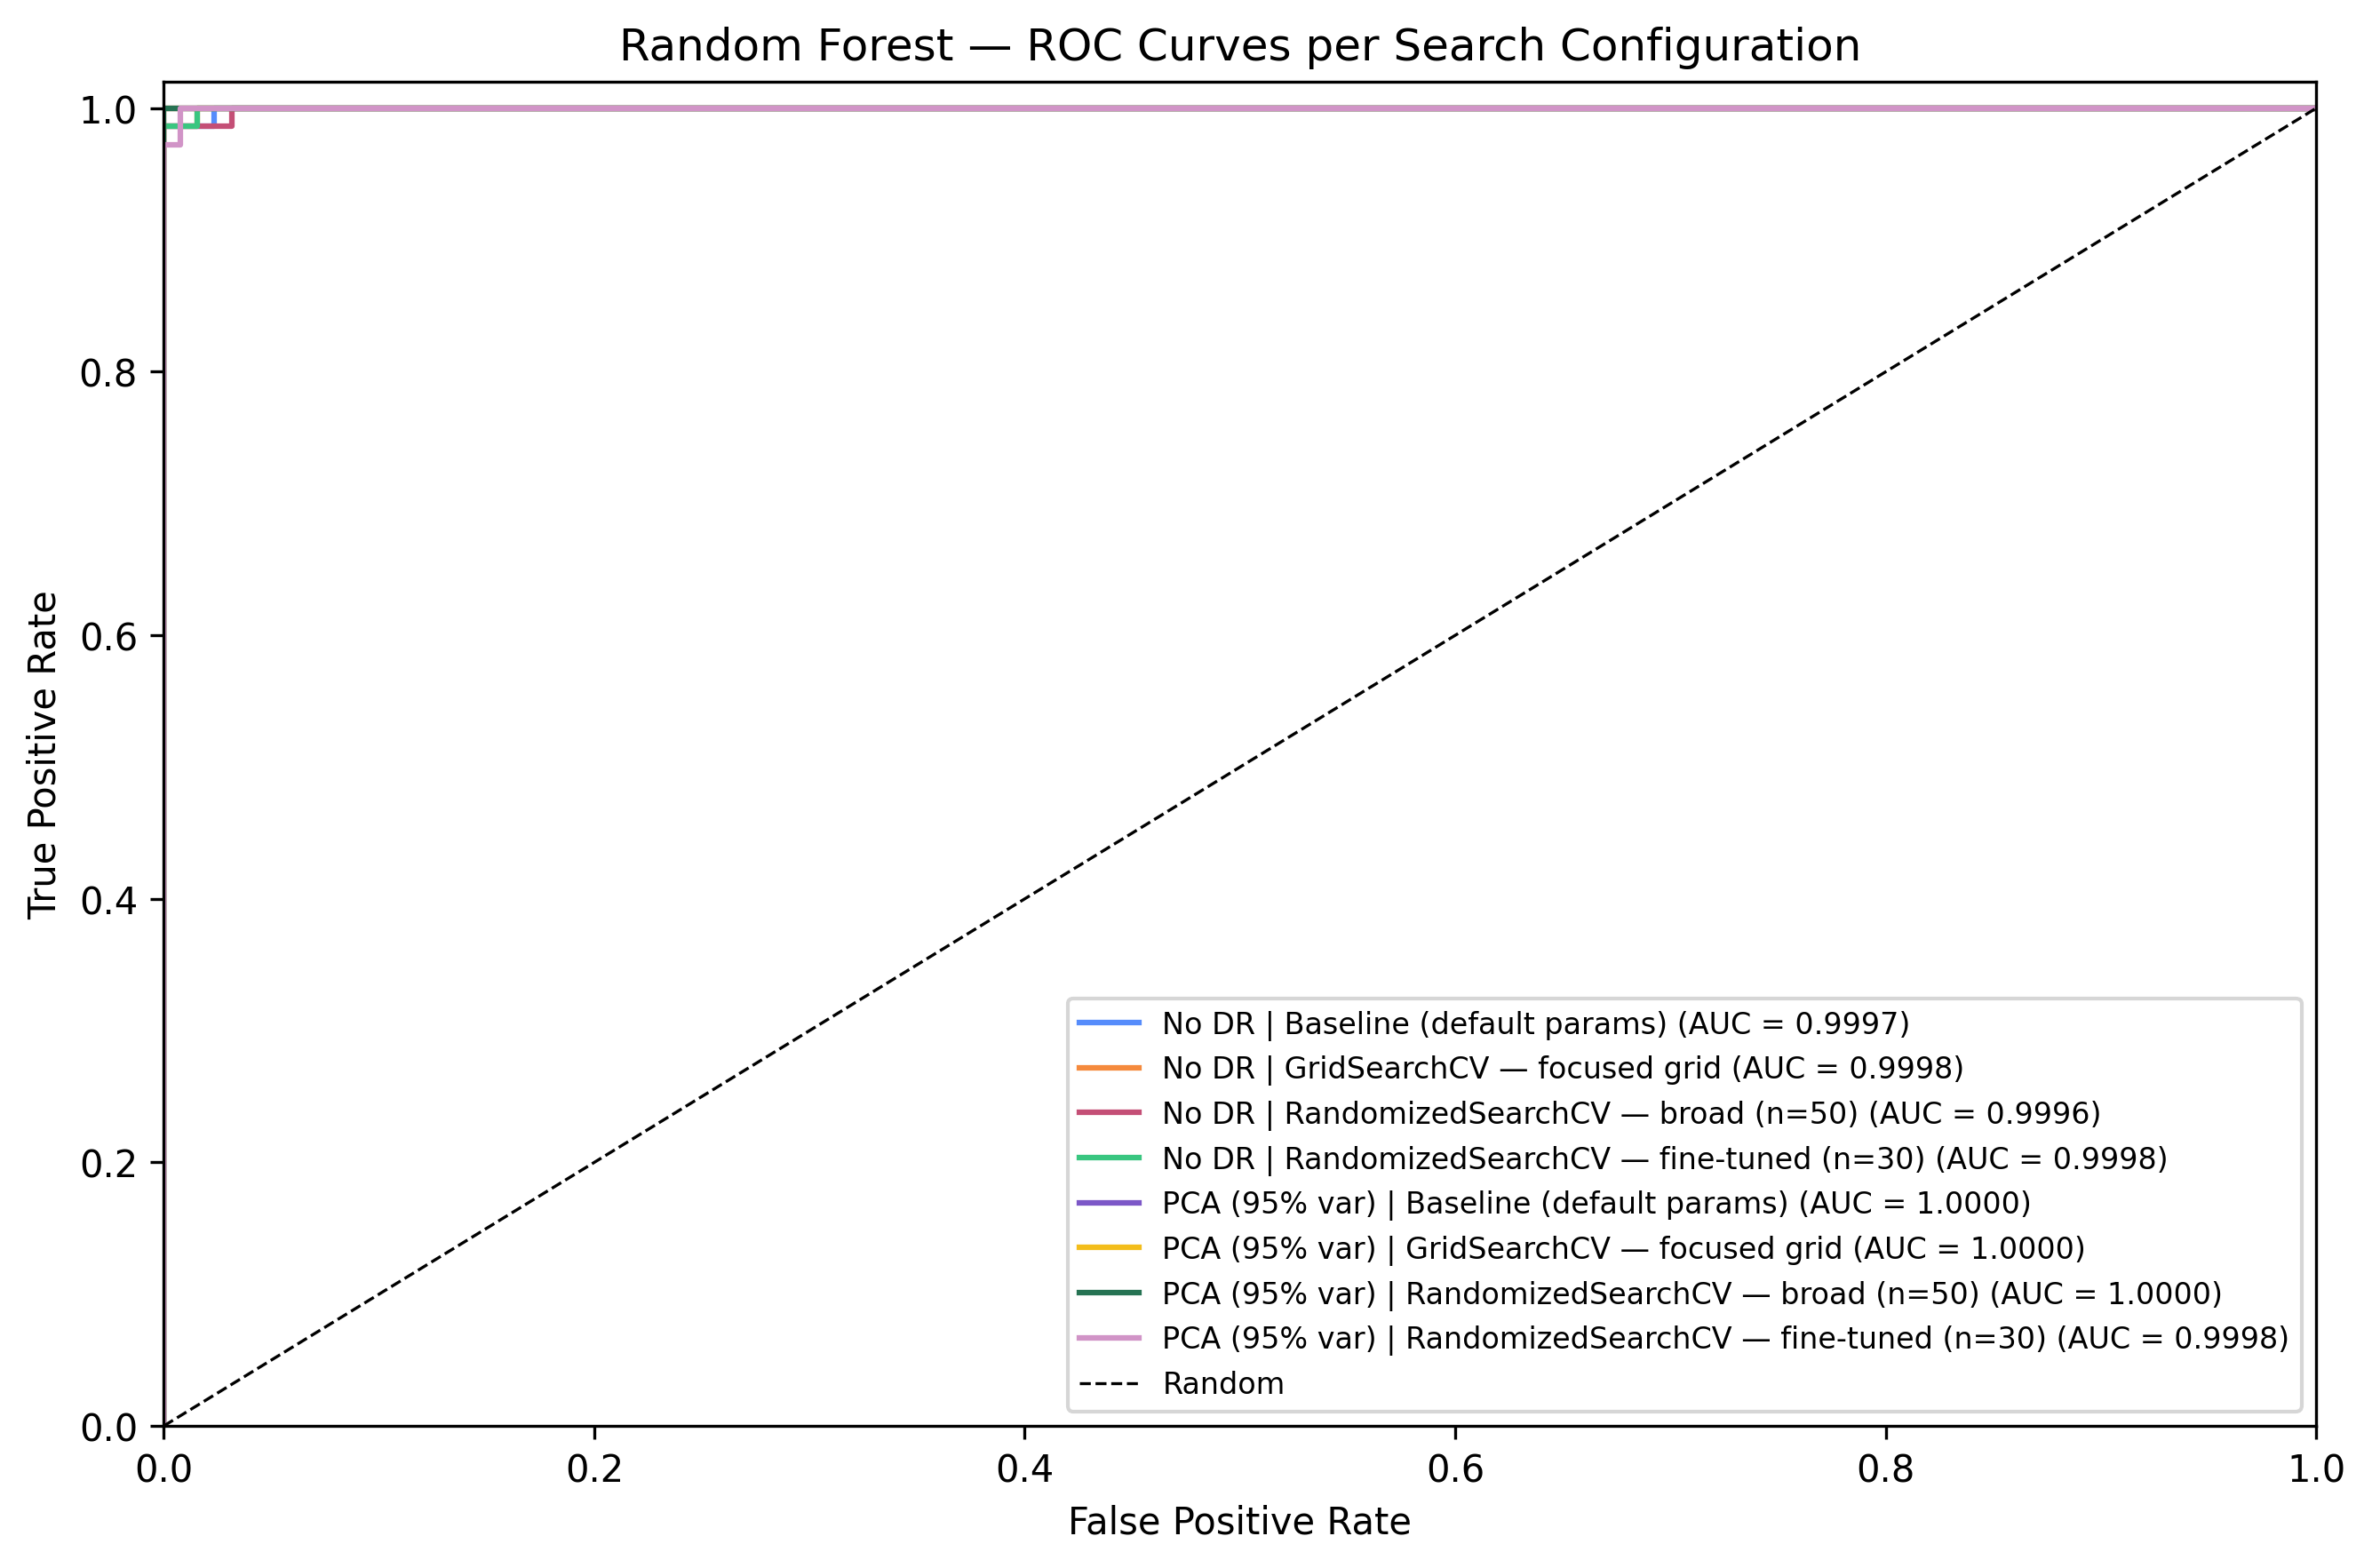
\includegraphics[width=\linewidth]{figures/optimize_rf_hyperparameters_roc_curve.png}
\caption{ROC curves.}
\end{subfigure}
\caption{Random Forest hyperparameter-tuning supporting plots.}
\label{fig:rf_hyperparameter_results}
\end{figure}

\FloatBarrier

\subsection{Explainability and Interpretation Results}

The explainability analysis was applied to the previously selected Random
Forest classifier. The goal of this stage was to interpret the selected model
after model selection, not to introduce a new model-selection criterion. The
analysis focused on the configured explained class \texttt{ckd}, so positive
SHAP values indicate increased support for this class and negative SHAP values
indicate reduced support for this class \cite{lundberg2017shap}.

Global interpretation combined native Random Forest feature importance,
permutation importance, and SHAP summaries. The resulting rankings highlighted
hematological, renal-function, and urine-related variables as relevant features
associated with model predictions. These rankings should be interpreted as
model-dependent predictive patterns rather than causal clinical effects. The
most relevant variables included hematological indicators such as hemo, pcv,
and rbcc; renal and urine-related attributes such as sg, grf, and al; and
clinical indicators such as htn, dm, and bgr. These correspond to hemoglobin,
packed cell volume, red blood cell count, specific gravity, glomerular
filtration rate, albumin, hypertension, diabetes mellitus, and blood glucose
random. Figure~\ref{fig:global_feature_importance_comparison} compares the
native feature-importance and permutation-importance views.

\begin{figure}[!htbp]
\centering
\begin{subfigure}{0.48\linewidth}
\centering
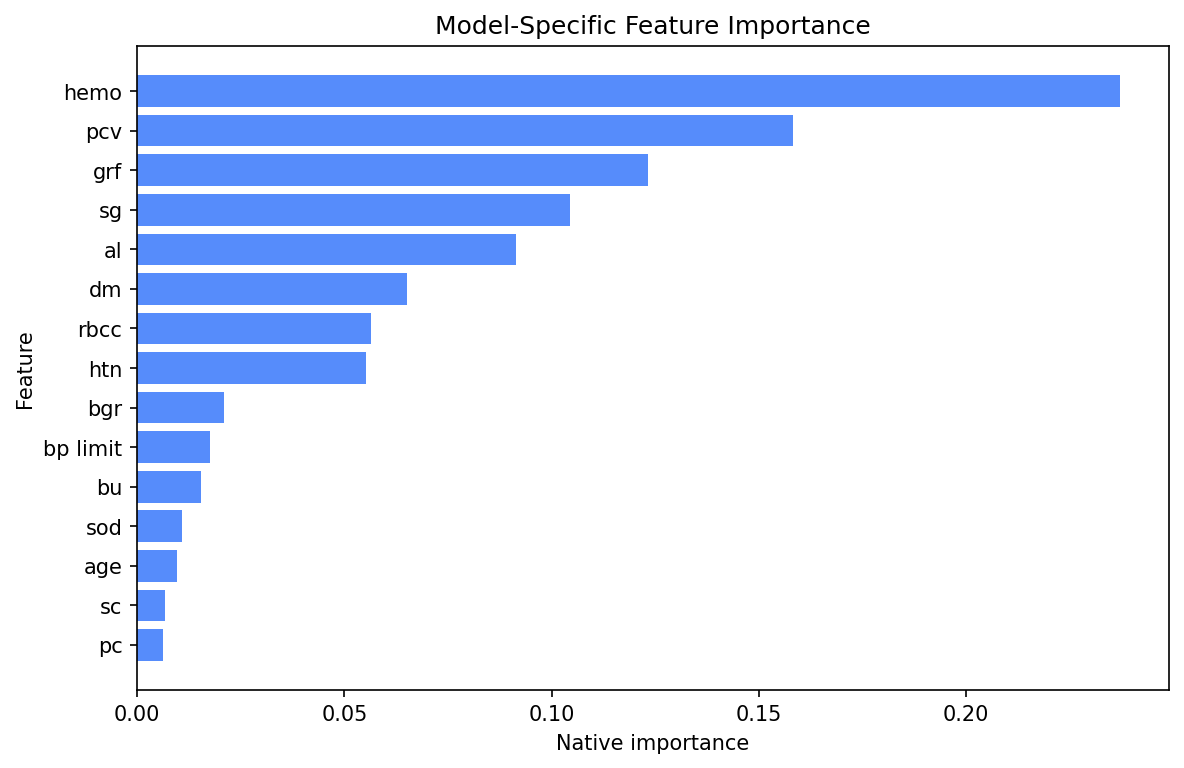
\includegraphics[width=\linewidth]{figures/native_feature_importance.png}
\caption{Model-specific feature importance.}
\label{fig:explainability_native_importance}
\end{subfigure}
\hfill
\begin{subfigure}{0.48\linewidth}
\centering
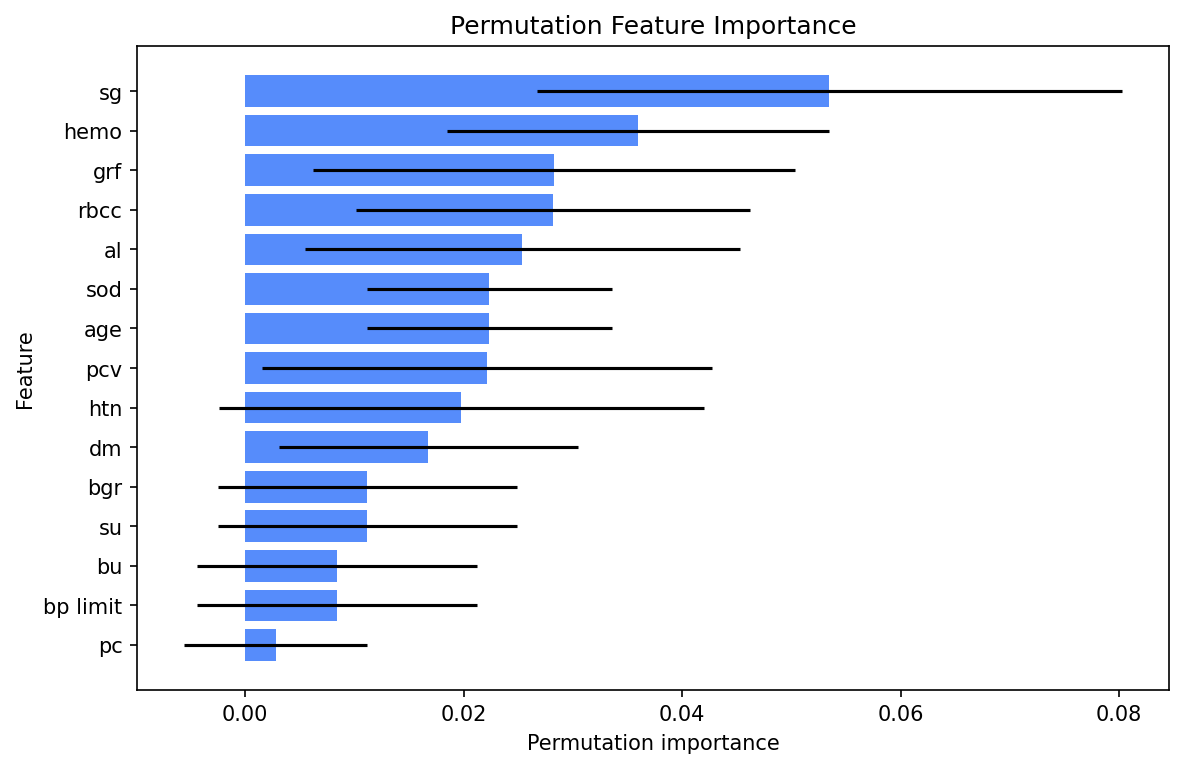
\includegraphics[width=\linewidth]{figures/permutation_importance.png}
\caption{Permutation feature importance.}
\label{fig:explainability_permutation_importance}
\end{subfigure}
\caption{Global feature-importance analysis for the selected Random Forest classifier.}
\label{fig:global_feature_importance_comparison}
\end{figure}

\FloatBarrier

SHAP summaries provided a complementary global interpretation of the selected
classifier. Figure~\ref{fig:global_shap_explanations} reports the mean absolute
SHAP values and the SHAP beeswarm summary for the explained class
\texttt{ckd} \cite{doshivelez2017interpretable,lundberg2017shap}.

\begin{figure}[!htbp]
\centering
\begin{subfigure}{0.48\linewidth}
\centering
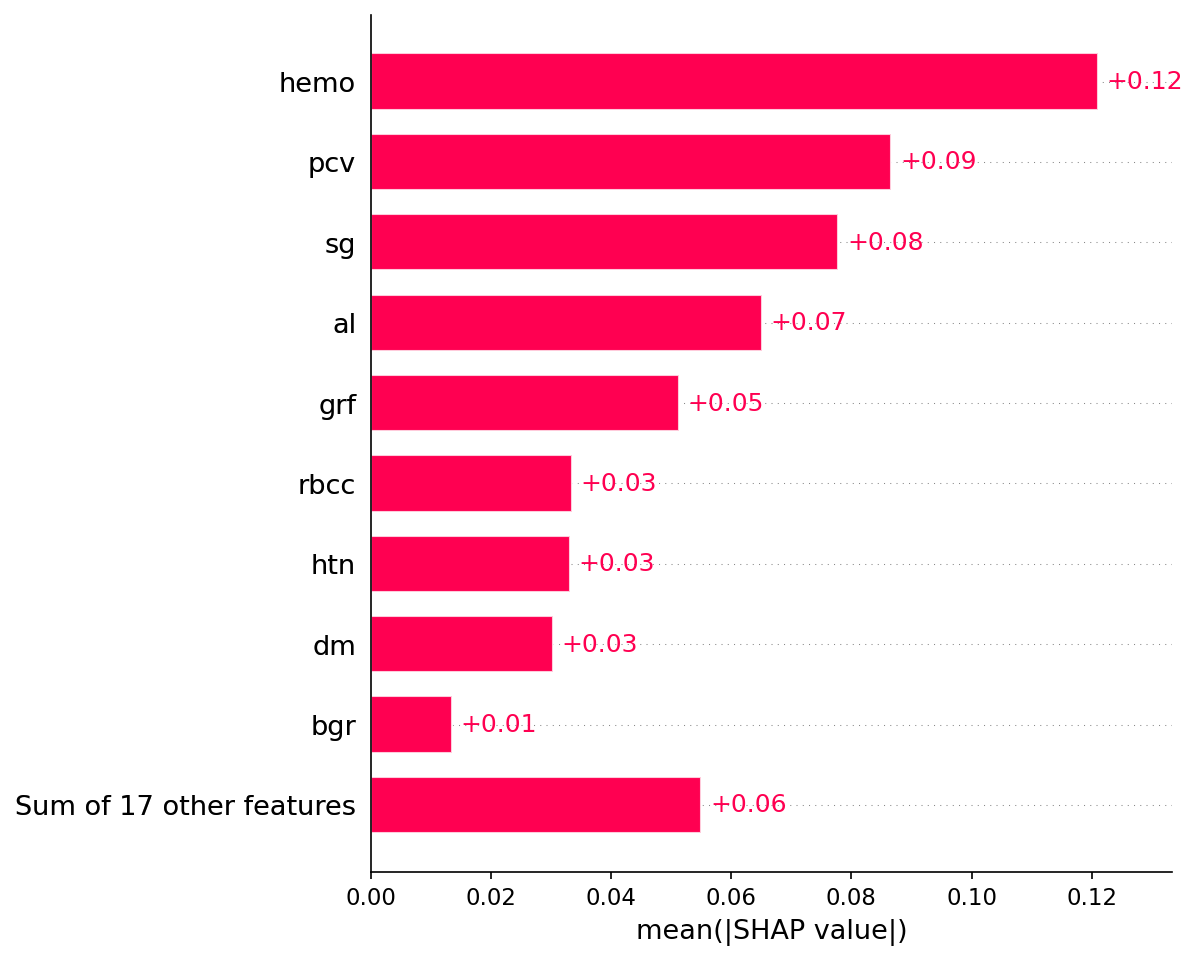
\includegraphics[width=\linewidth]{figures/shap_global_bar.png}
\caption{Mean absolute SHAP values.}
\label{fig:explainability_shap_global_bar}
\end{subfigure}
\hfill
\begin{subfigure}{0.48\linewidth}
\centering
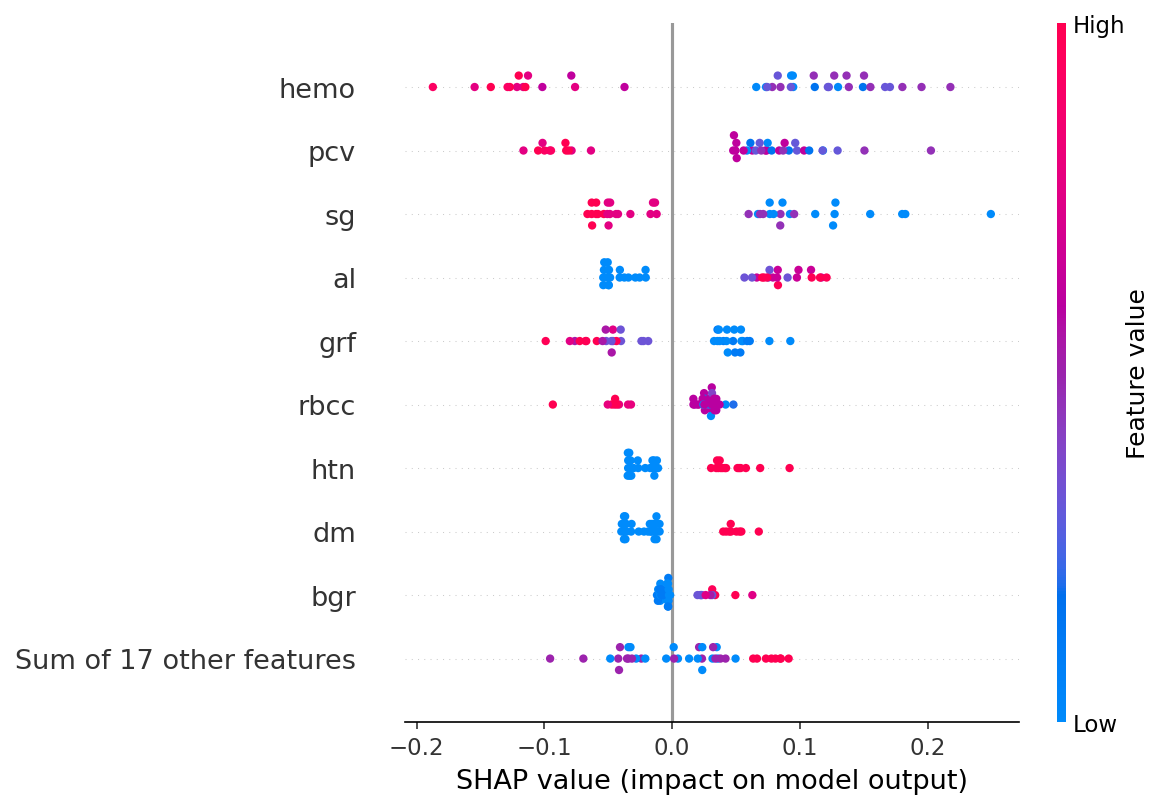
\includegraphics[width=\linewidth]{figures/shap_beeswarm.png}
\caption{SHAP beeswarm summary.}
\label{fig:explainability_shap_beeswarm}
\end{subfigure}
\caption{Global SHAP explanations for the configured explained class, \texttt{ckd}.}
\label{fig:global_shap_explanations}
\end{figure}

\FloatBarrier

Local explanations were generated for representative test instances using SHAP
waterfall plots and LIME. The LIME outputs were exported as local HTML and CSV
artifacts and used as complementary local explanations
\cite{ribeiro2016lime}. Figure~\ref{fig:local_shap_waterfall_explanations}
shows the local SHAP waterfall explanations included in the paper.

\begin{figure}[!htbp]
\centering
\begin{subfigure}{0.46\linewidth}
\centering
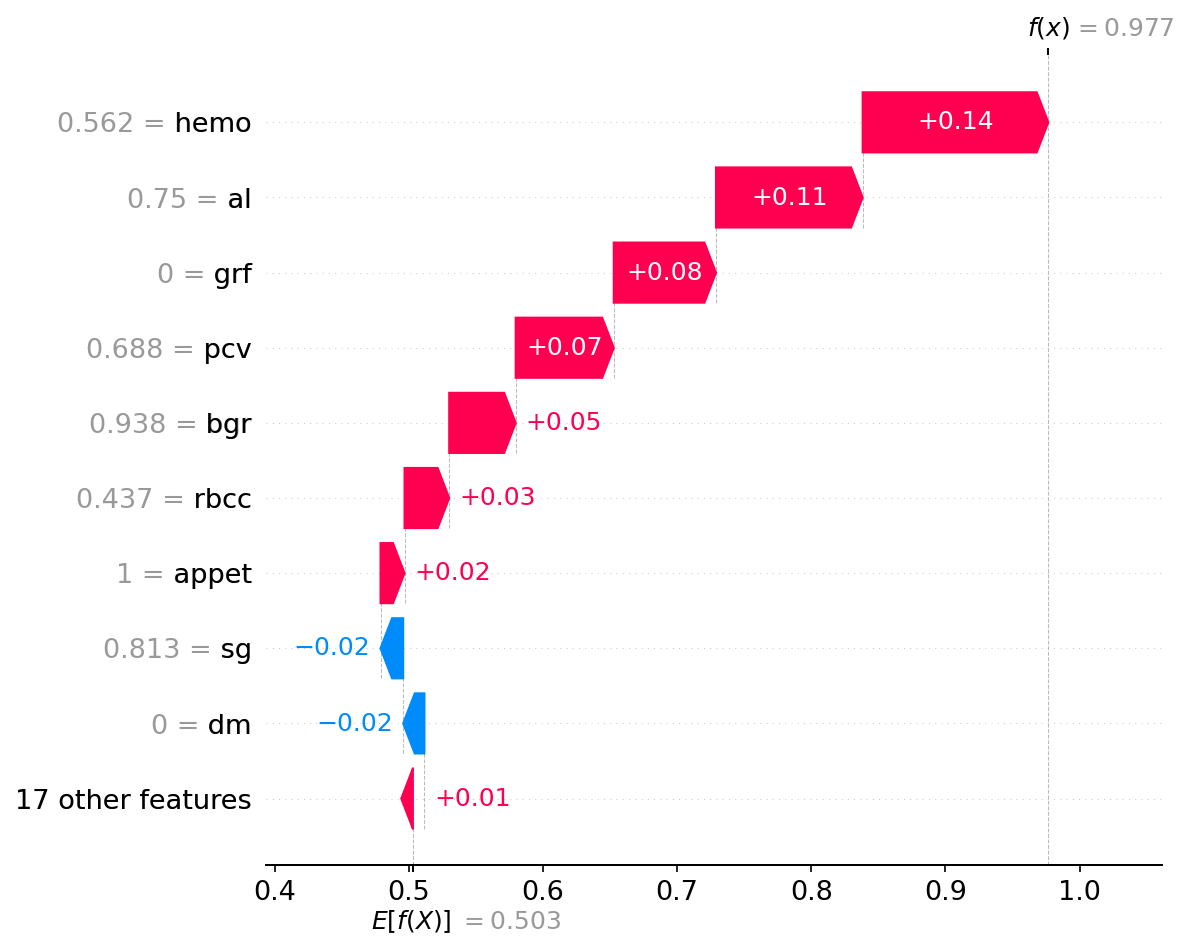
\includegraphics[width=\linewidth]{figures/shap_waterfall_instance_0.png}
\caption{Representative instance.}
\label{fig:explainability_shap_waterfall_instance_0}
\end{subfigure}
\hfill
\begin{subfigure}{0.46\linewidth}
\centering
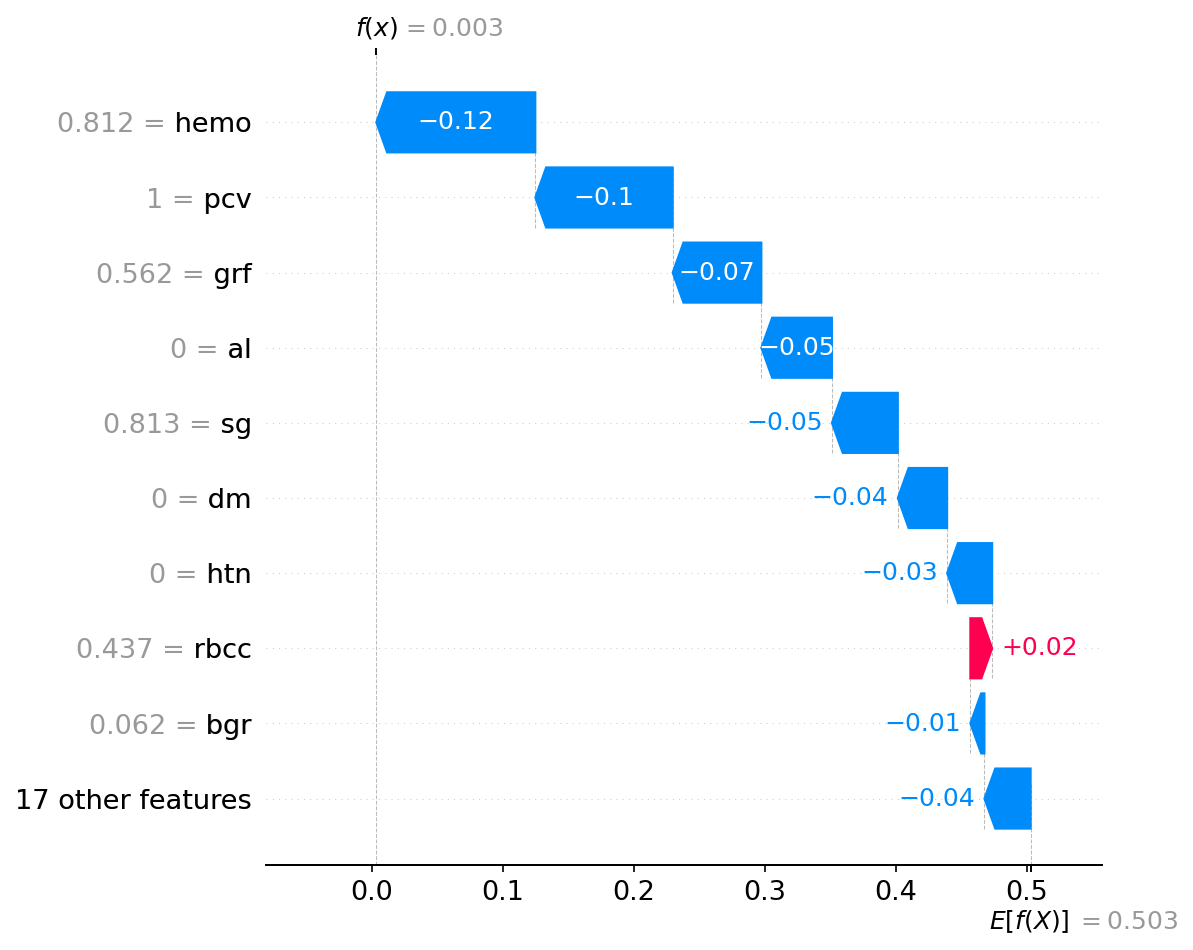
\includegraphics[width=\linewidth]{figures/shap_waterfall_instance_4.png}
\caption{Second representative instance.}
\label{fig:explainability_shap_waterfall_instance_4}
\end{subfigure}
\caption{Local SHAP waterfall explanations for representative test instances.}
\label{fig:local_shap_waterfall_explanations}
\end{figure}

\FloatBarrier


\section{Conclusion}

Regarding the exploration over Calancing Spot Checking, four different approaches were tested: No Ballancing, SMOTE, Random Under Sampler and SMOTE+TomekLinks.
As initially said, the data without balancing effort was on a 64\%-36\% distribution, which is a faily even distribution. The three balancing technique results had minor impact on the model quality,
proving data distribution is enough for proper ML modeling on the different models evaluated.
The dimensionality reduction and feature selection experiments demonstrated that reducing the feature space can improve both model performance and stability.
We've tried different types of dimention reduction and PCA achieved the best overall results. The wrapper-based selection showed slightly lower performance.
Results indicate that dimensionality reduction contributed positively.

\todo{
\begin{itemize}
    \item Summarize the main objectives and outcomes of the study.
    \item Highlight the best-performing models and the most relevant findings.
    \item Discuss the practical implications of the results.
    \item Identify limitations of the study.
    \item Suggest possible improvements and directions for future work.
\end{itemize}
}

% ===== References =====
\section{References}
\bibliographystyle{sbc}
\bibliography{references}

\end{document}
